%-----------------------------------------------------------------------------
% Beginning of appendix1.tex
%-----------------------------------------------------------------------------
%
%%%%%%%%%%%%%%%%%%%%%%%%%%%%%%%%%%%%%%%%%%%%%%%%%%%%%%%%%%%%%%%%%%%%%%%%

\chapter{APPENDIX A}

\section{Metabolism Data}

Below are graphs of temporal variation for all sites for GPP (green lines), ER (orange lines), and NEP (black lines) across the coupled gradients. Sites are arranged arid to mesic top down. 


\begin{figure}[htb]
\begin{center}
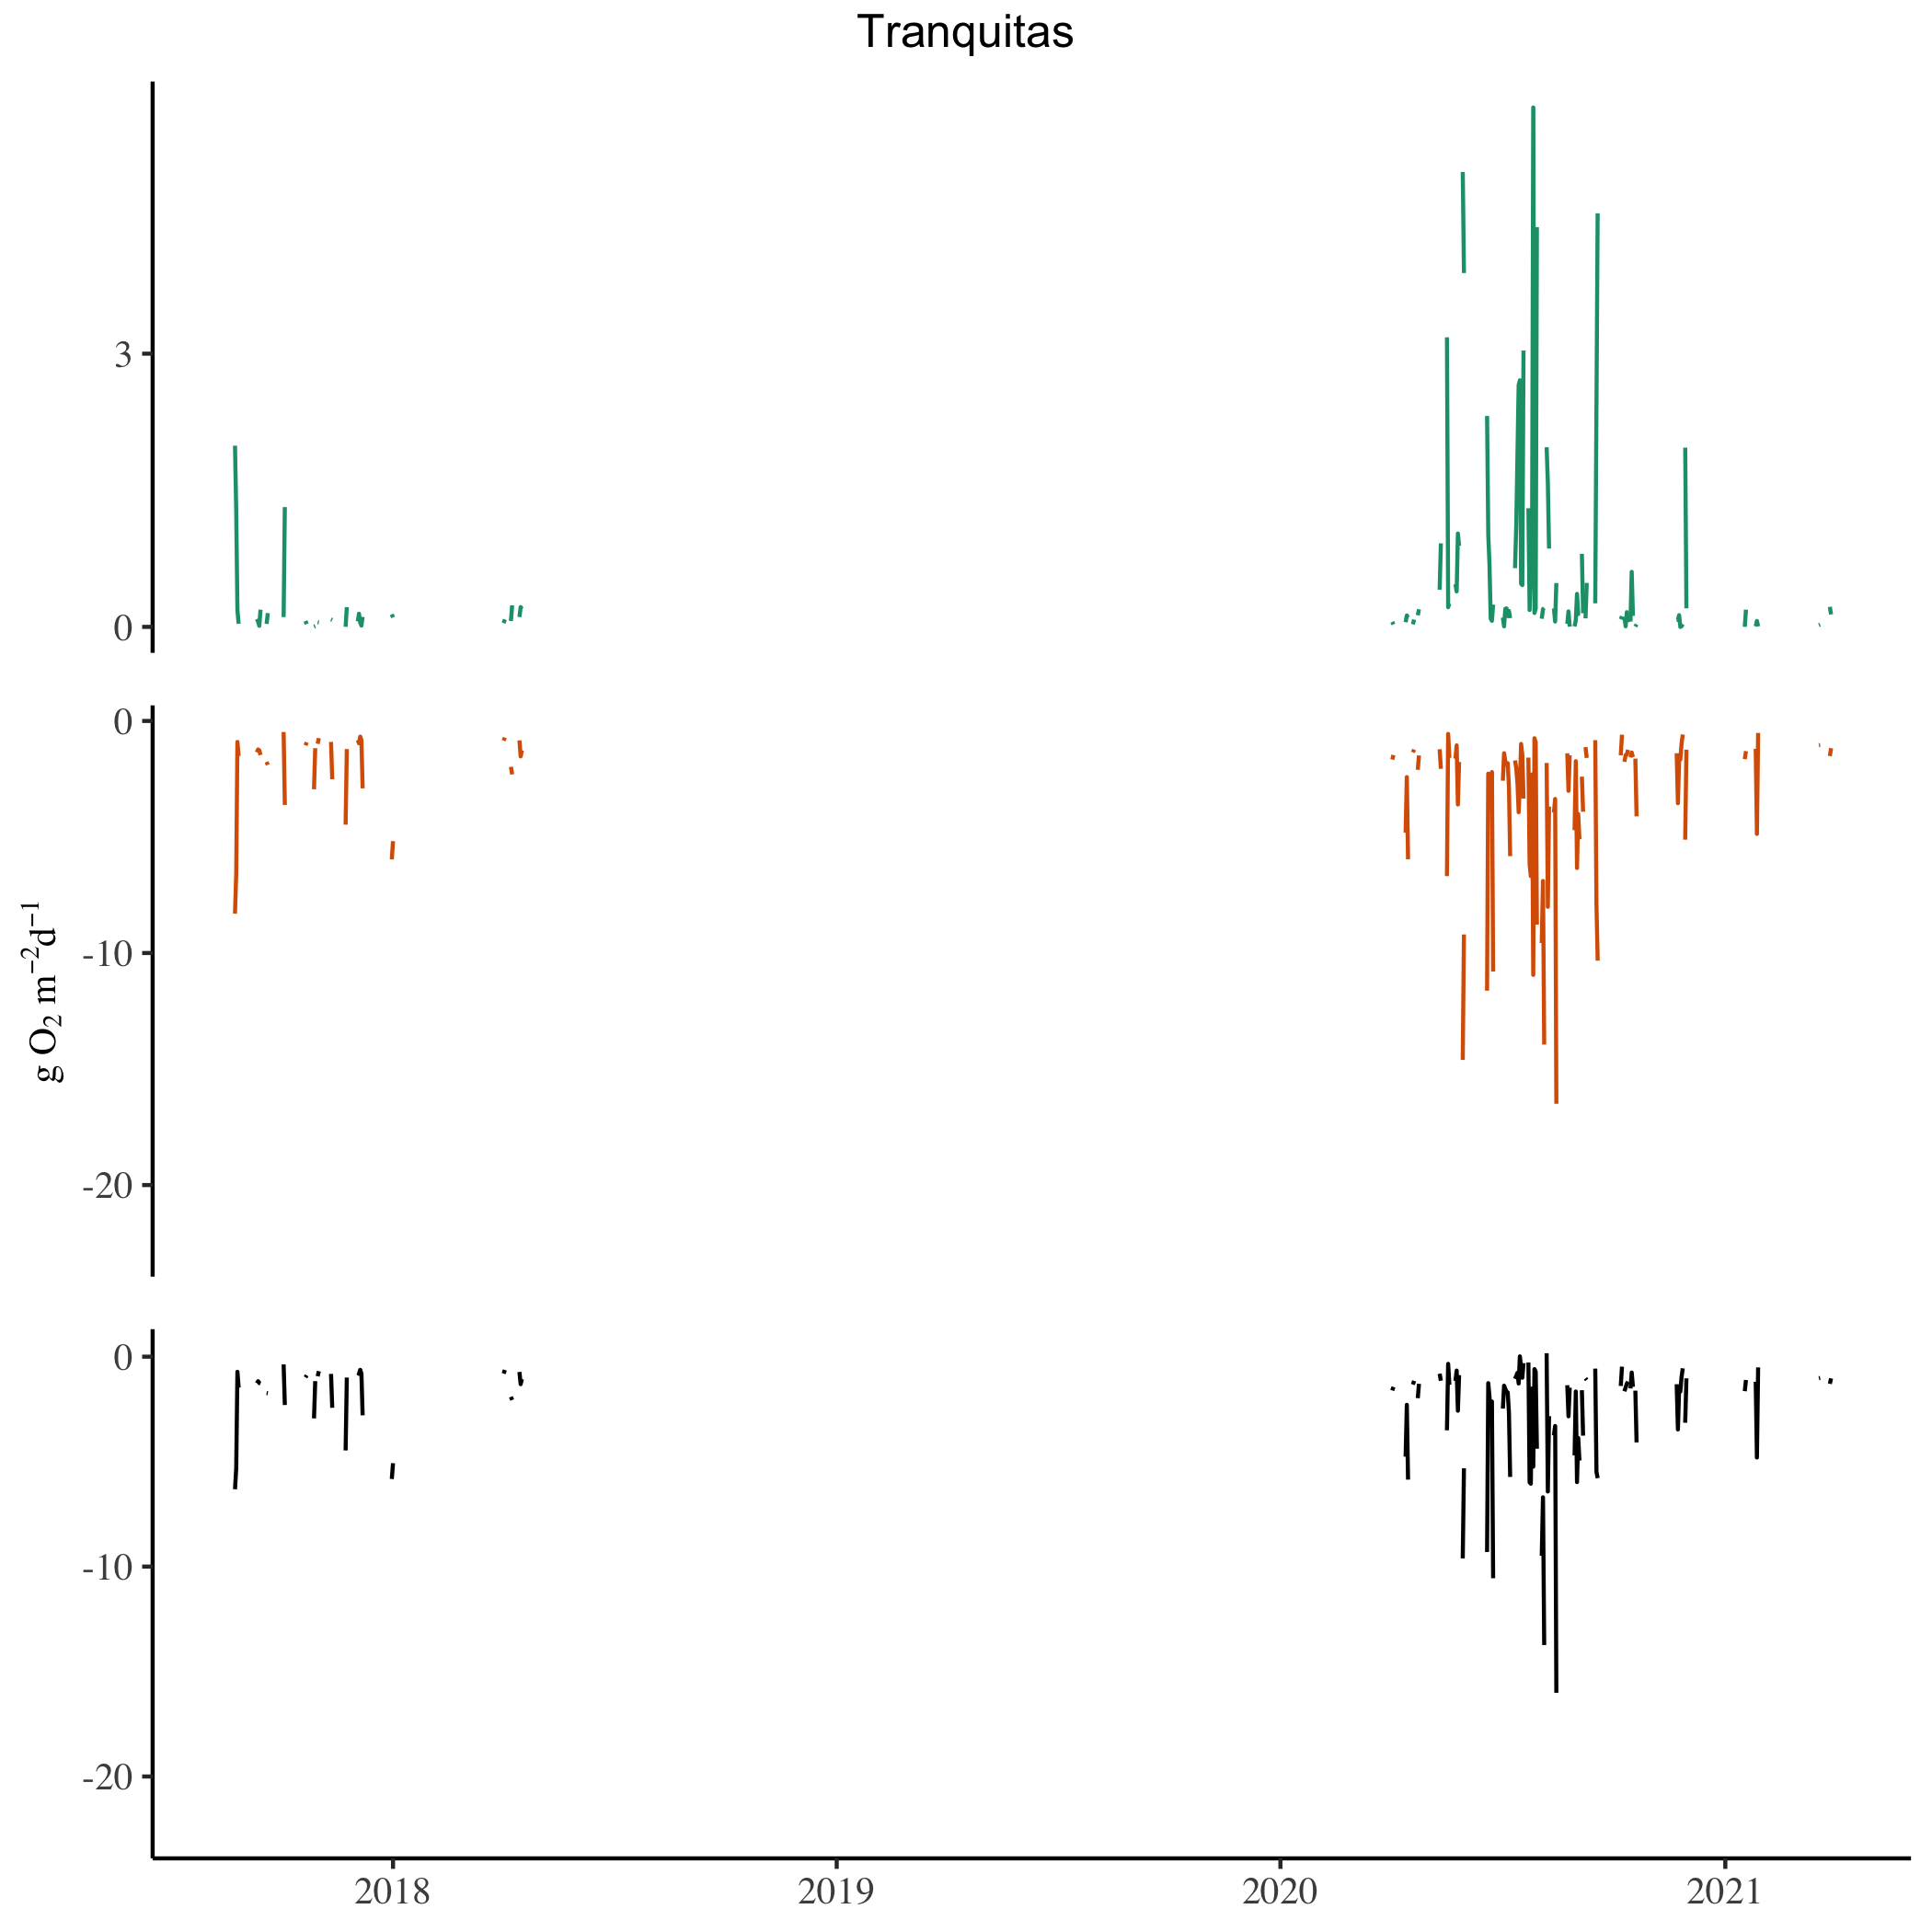
\includegraphics[scale=0.2]{Figs/TRC.png}
\caption{Tranquitas Creek.}
\label{Fig:TRC}
\end{center}
\end{figure}

\begin{figure}[htb]
\begin{center}
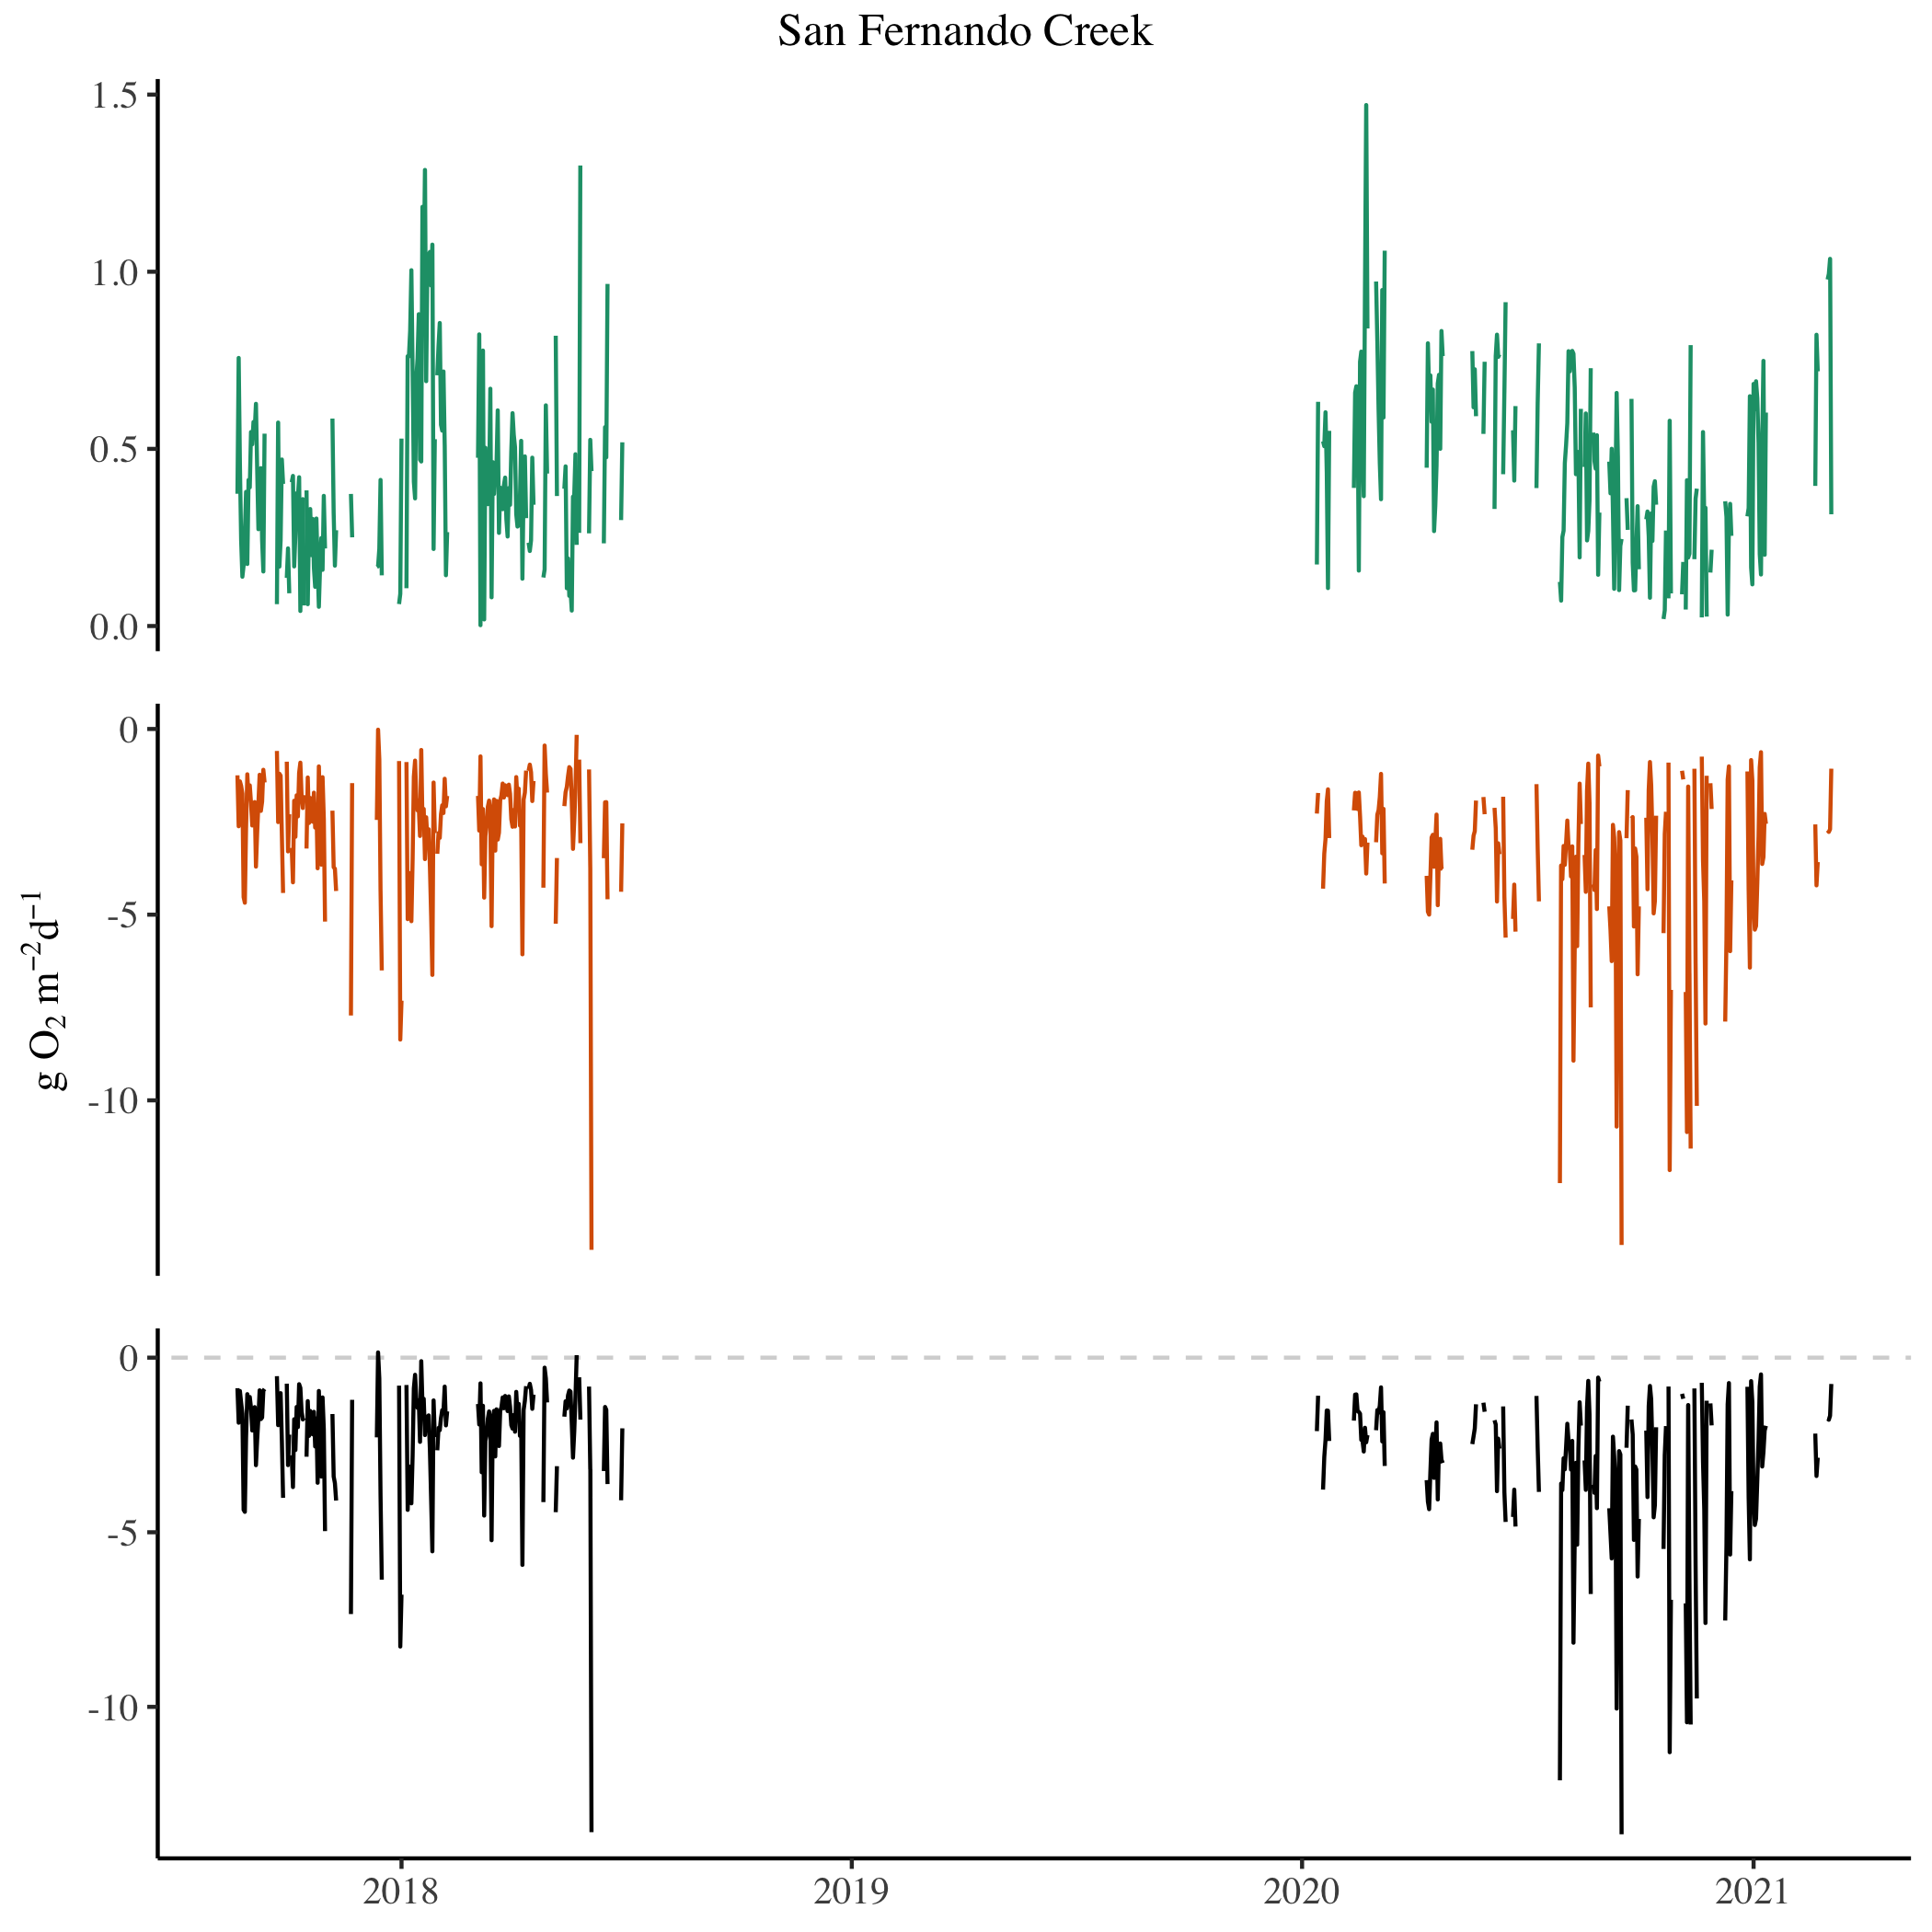
\includegraphics[scale=0.2]{Figs/SFC.png}
\caption{San Fernando Creek}
\label{Fig:SFC}
\end{center}
\end{figure}

\begin{figure}[htb]
\begin{center}
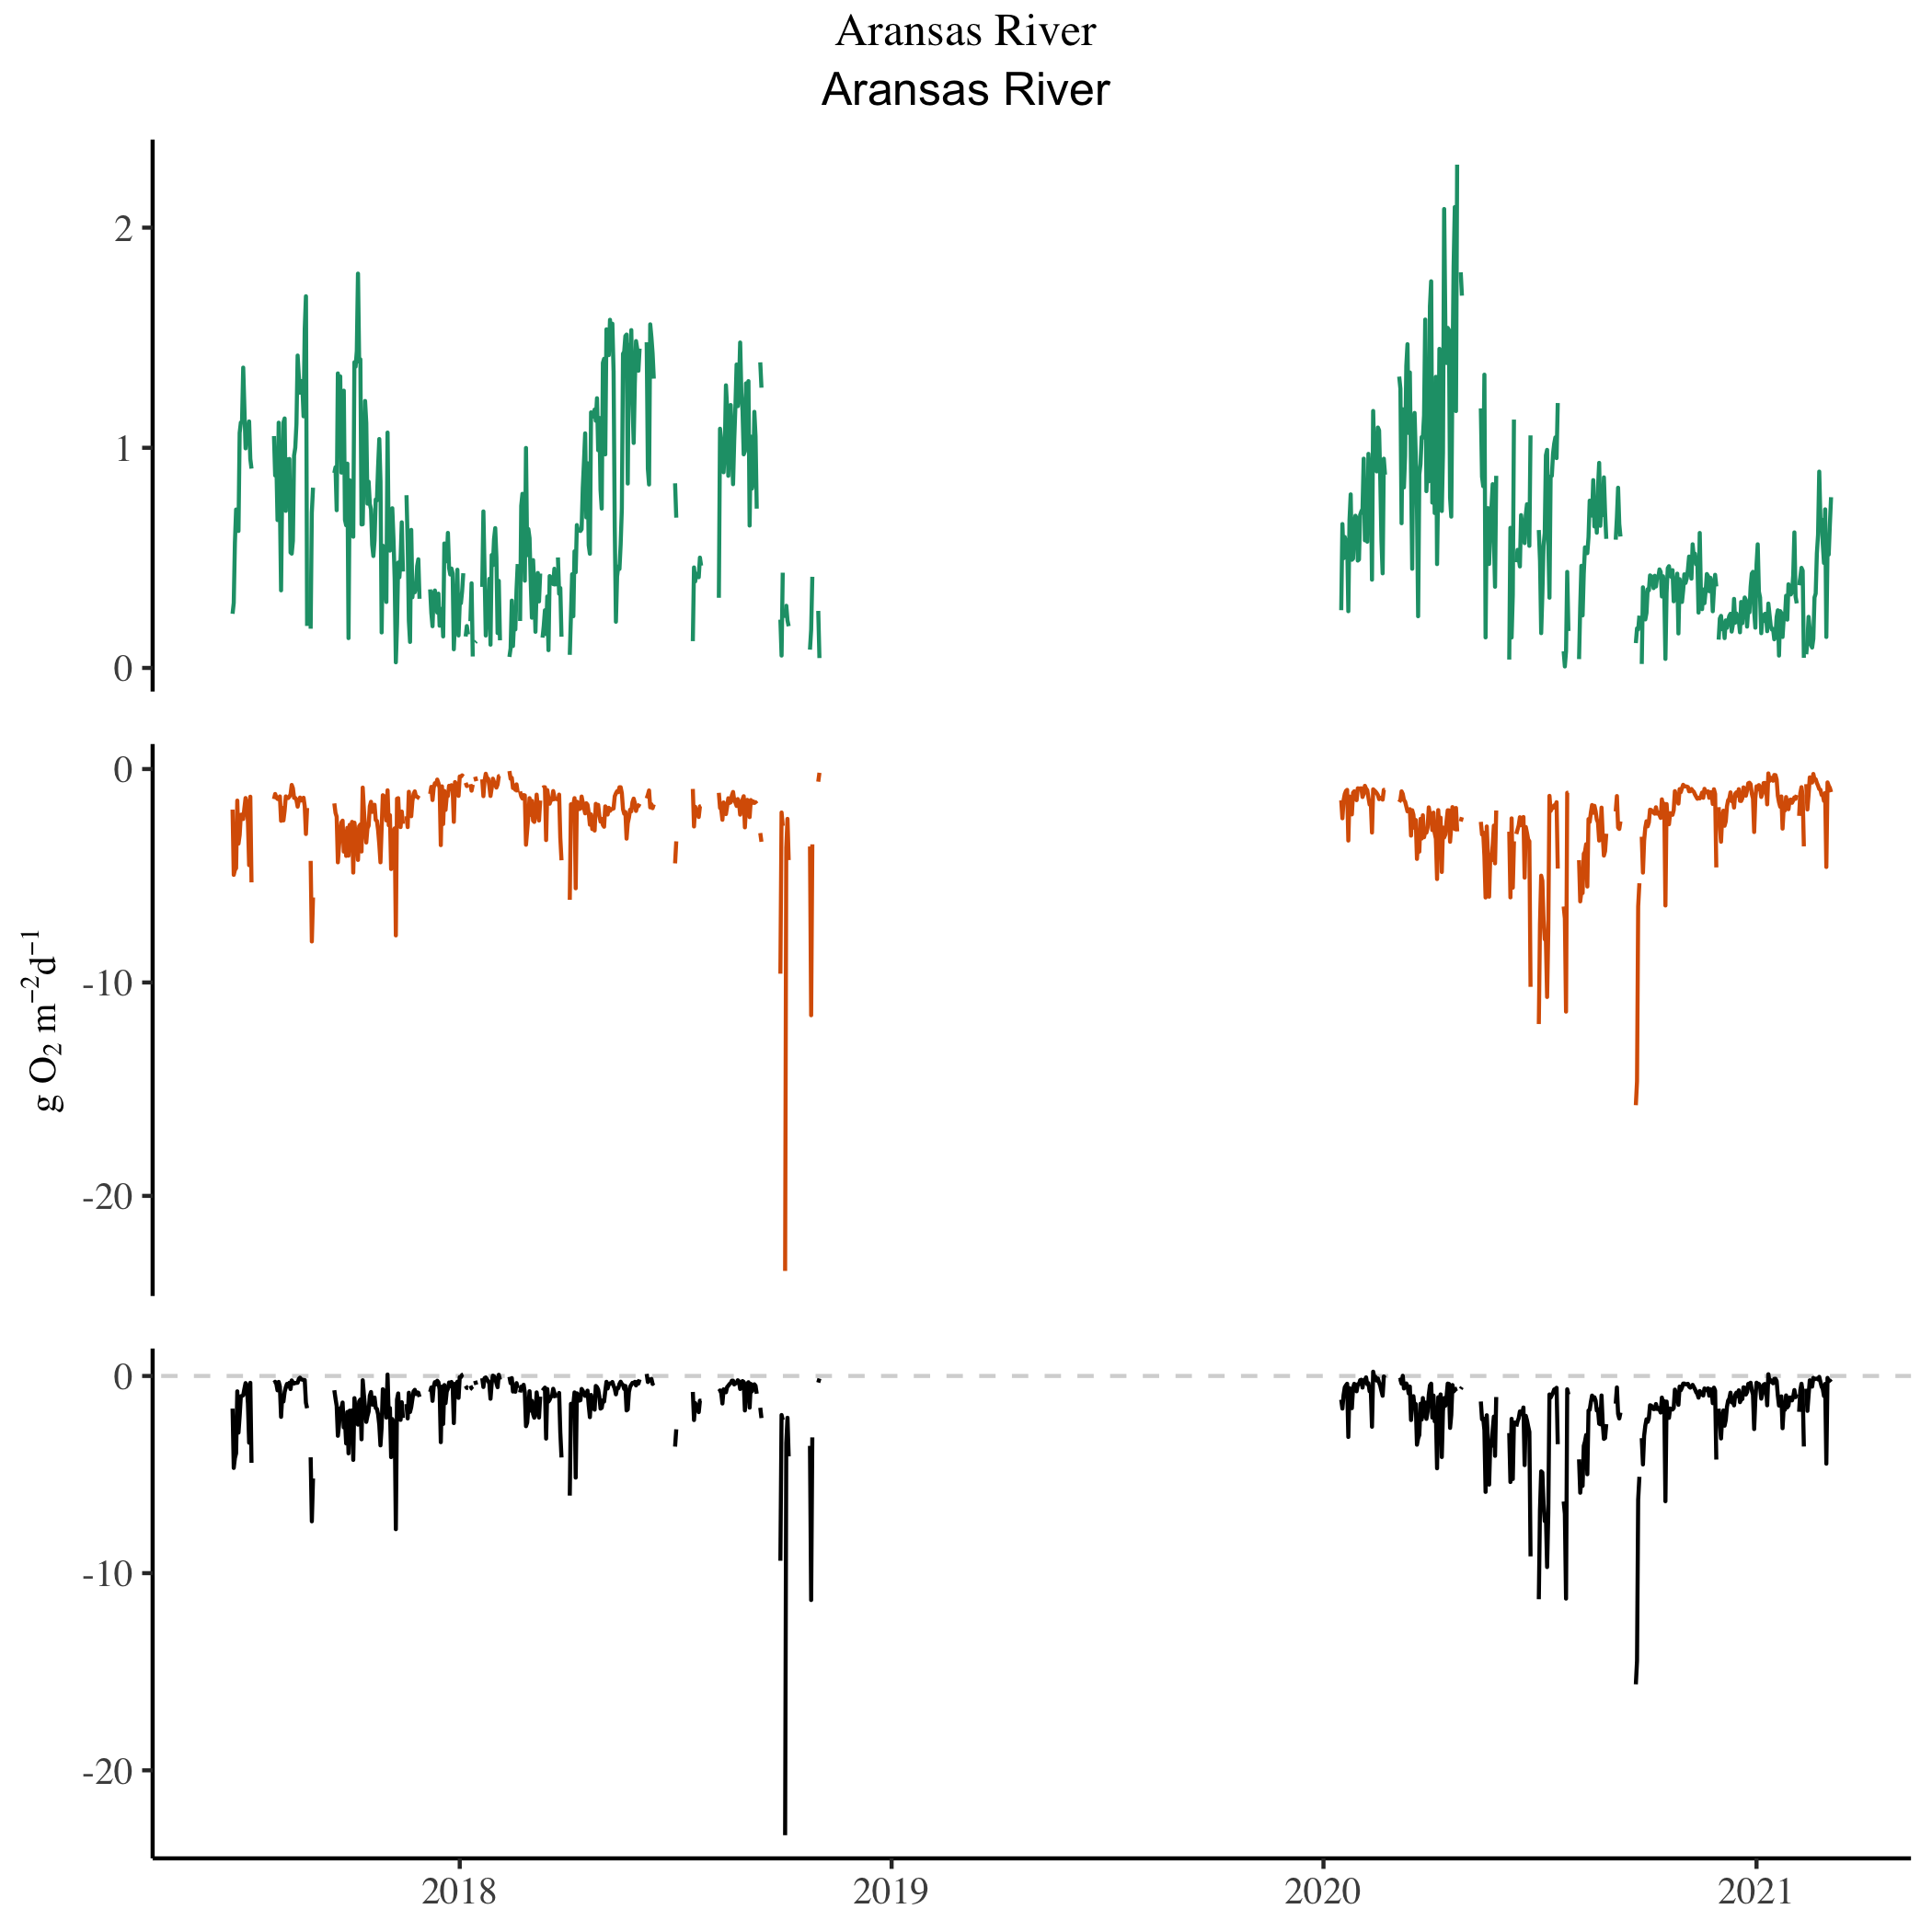
\includegraphics[scale=0.2]{Figs/AR.png}
\caption{Aransas River}
\label{Fig:AR}
\end{center}
\end{figure}

\begin{figure}[htb]
\begin{center}
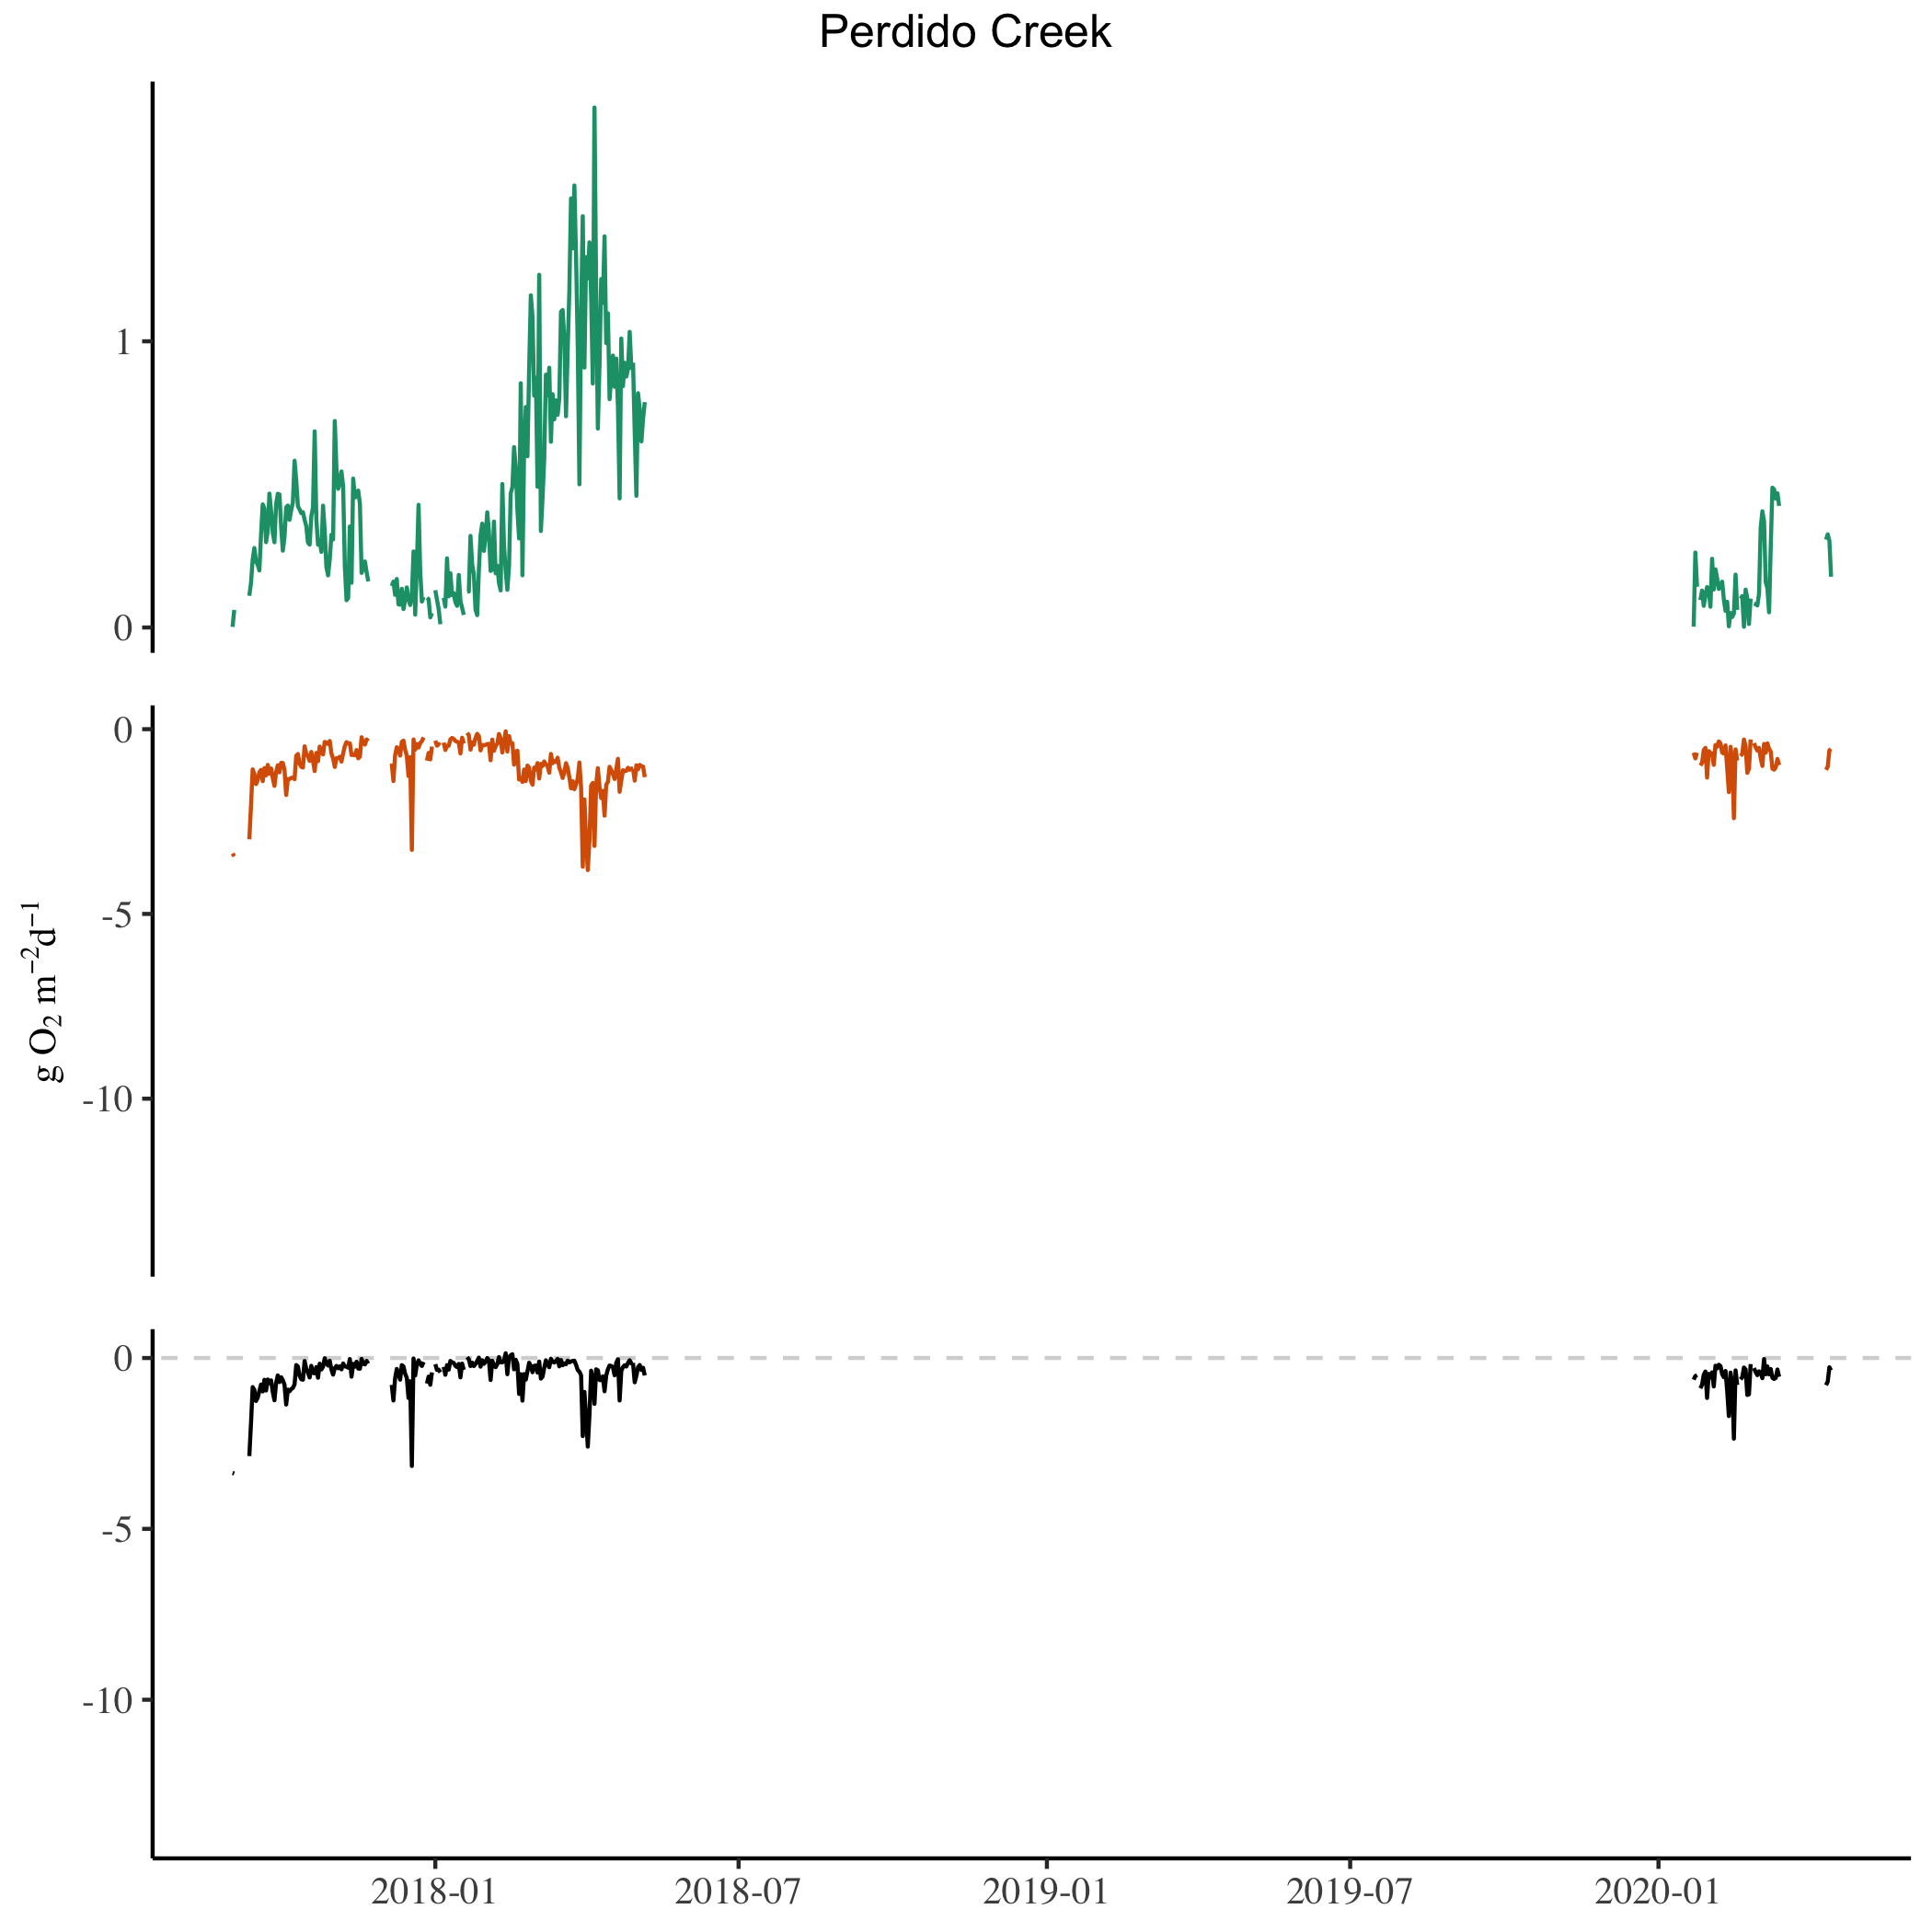
\includegraphics[scale=0.2]{Figs/PDC.png}
\caption{Perdido Creek}
\label{Fig:PDC}
\end{center}
\end{figure}

\begin{figure}[htb]
\begin{center}
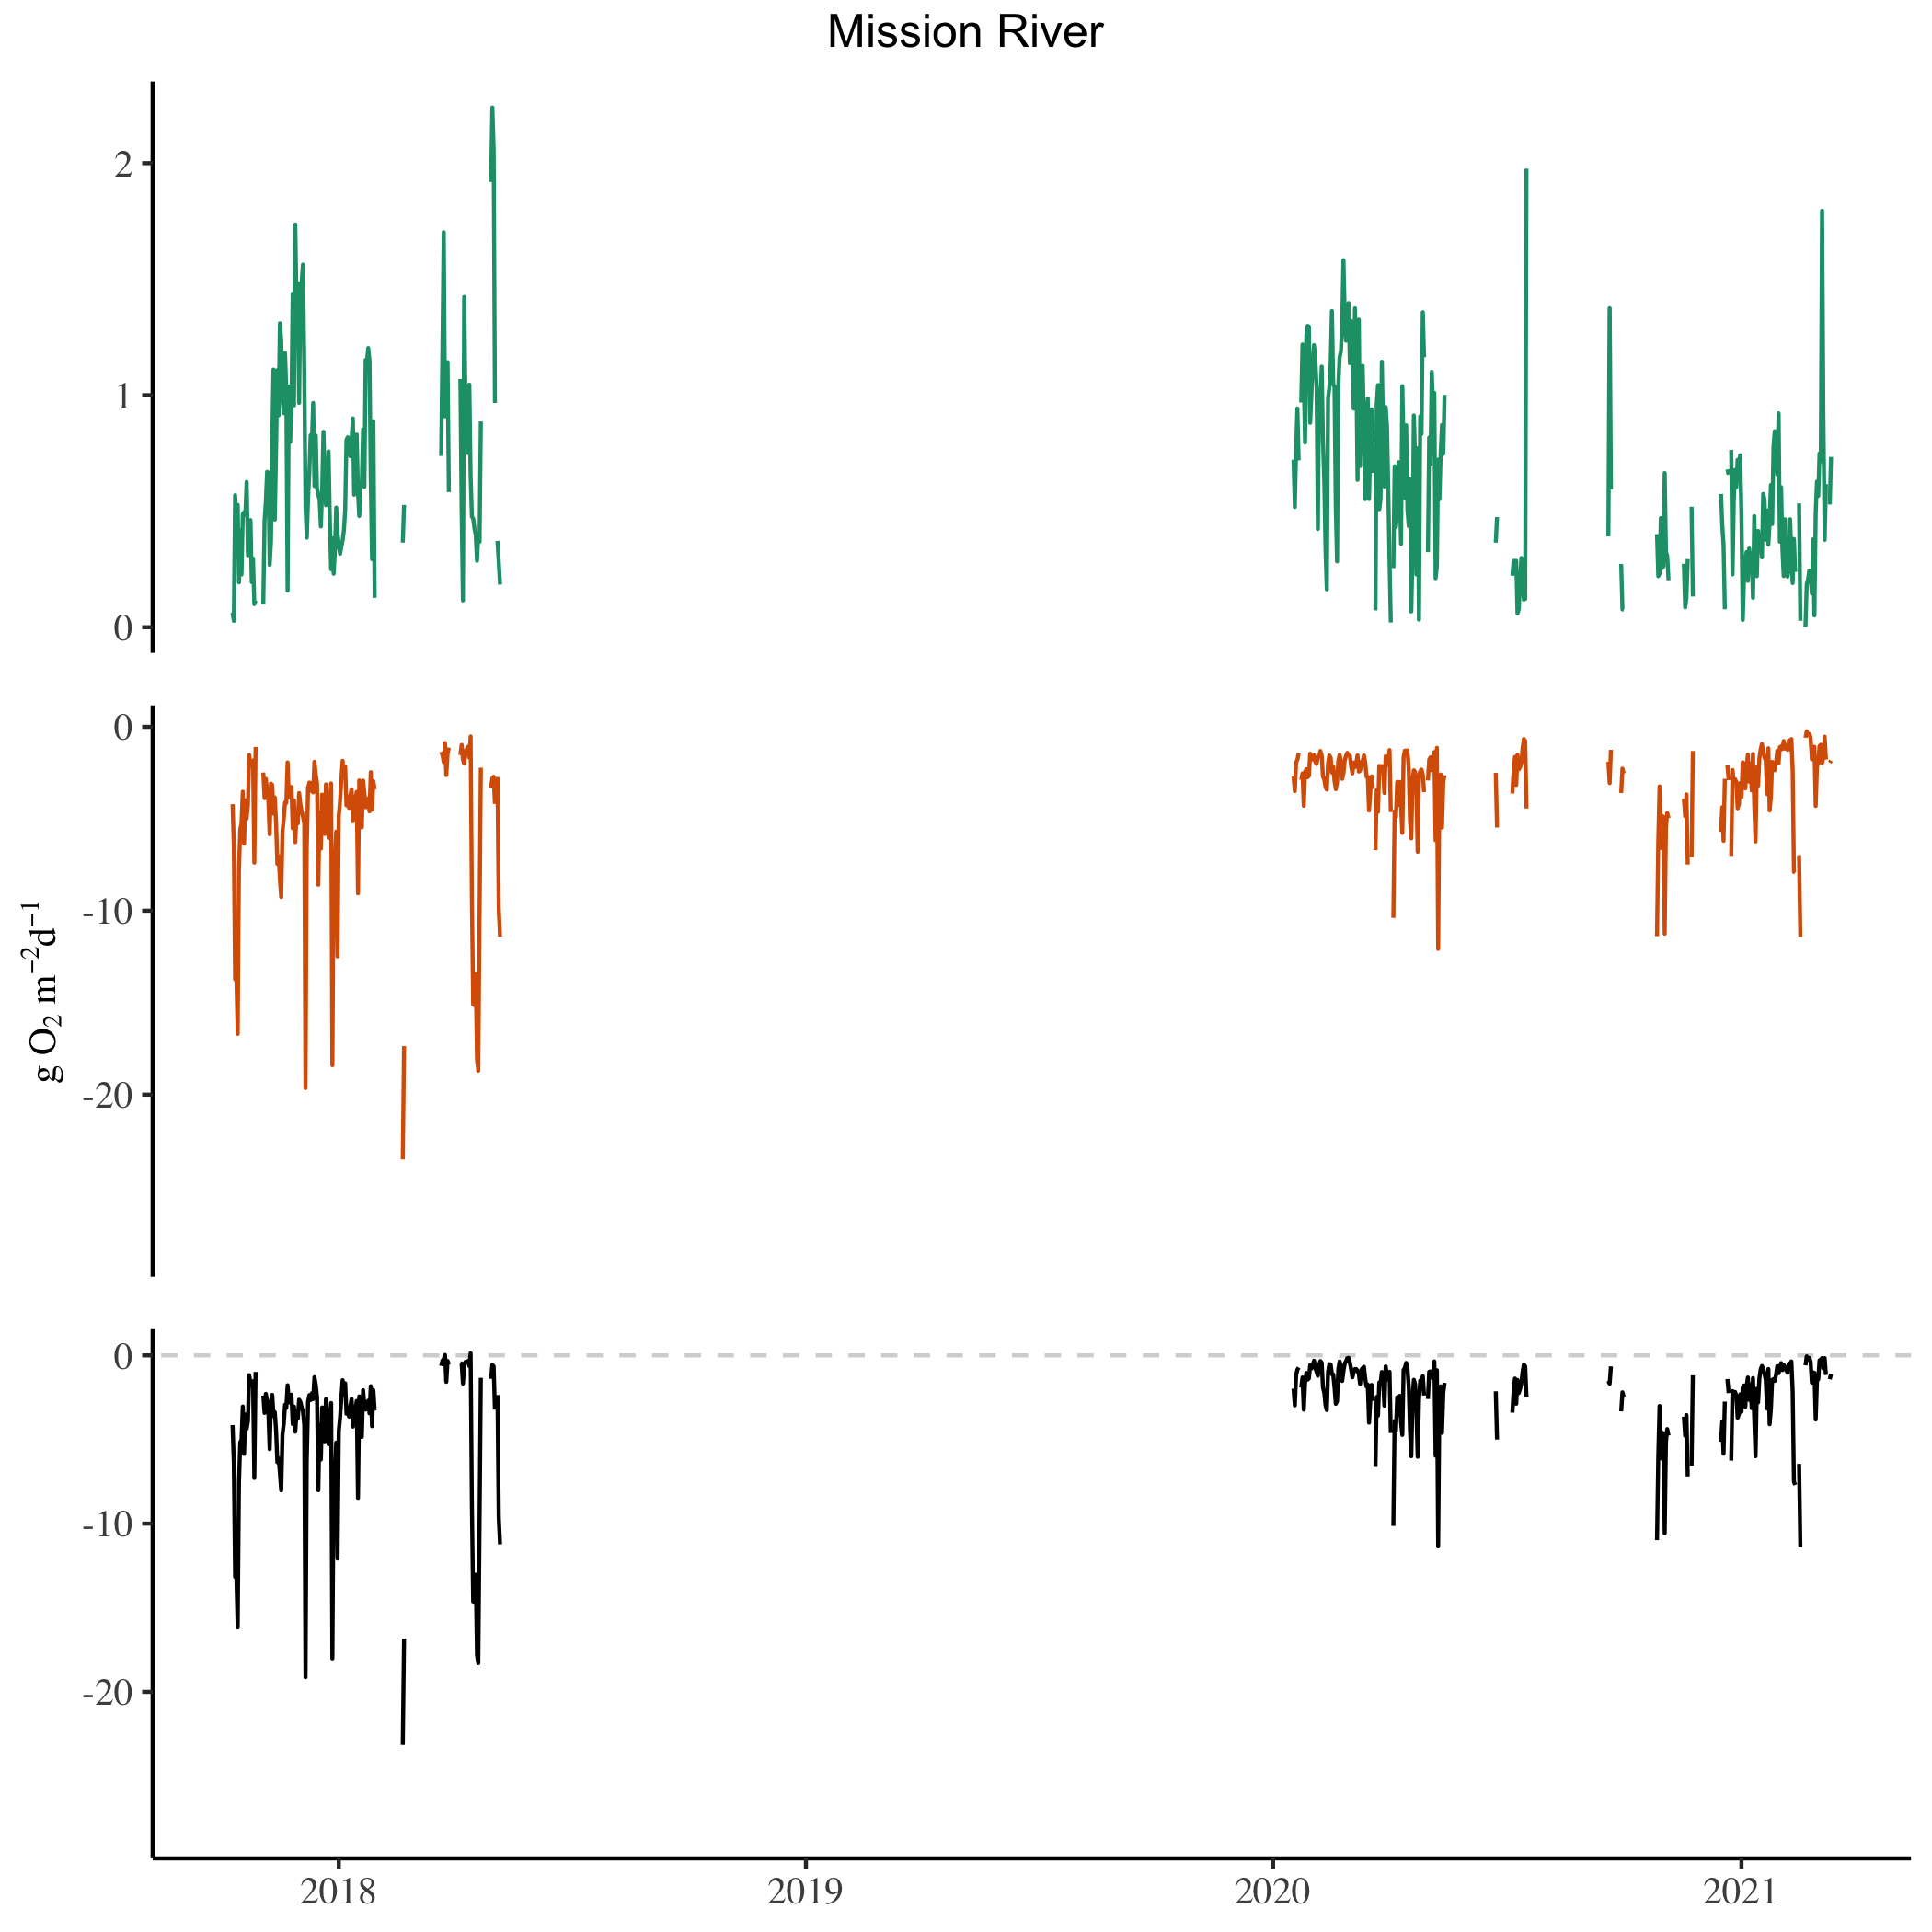
\includegraphics[scale=0.2]{Figs/MR.png}
\caption{Mission River}
\label{Fig:MR}
\end{center}
\end{figure}

\begin{figure}[htb]
\begin{center}
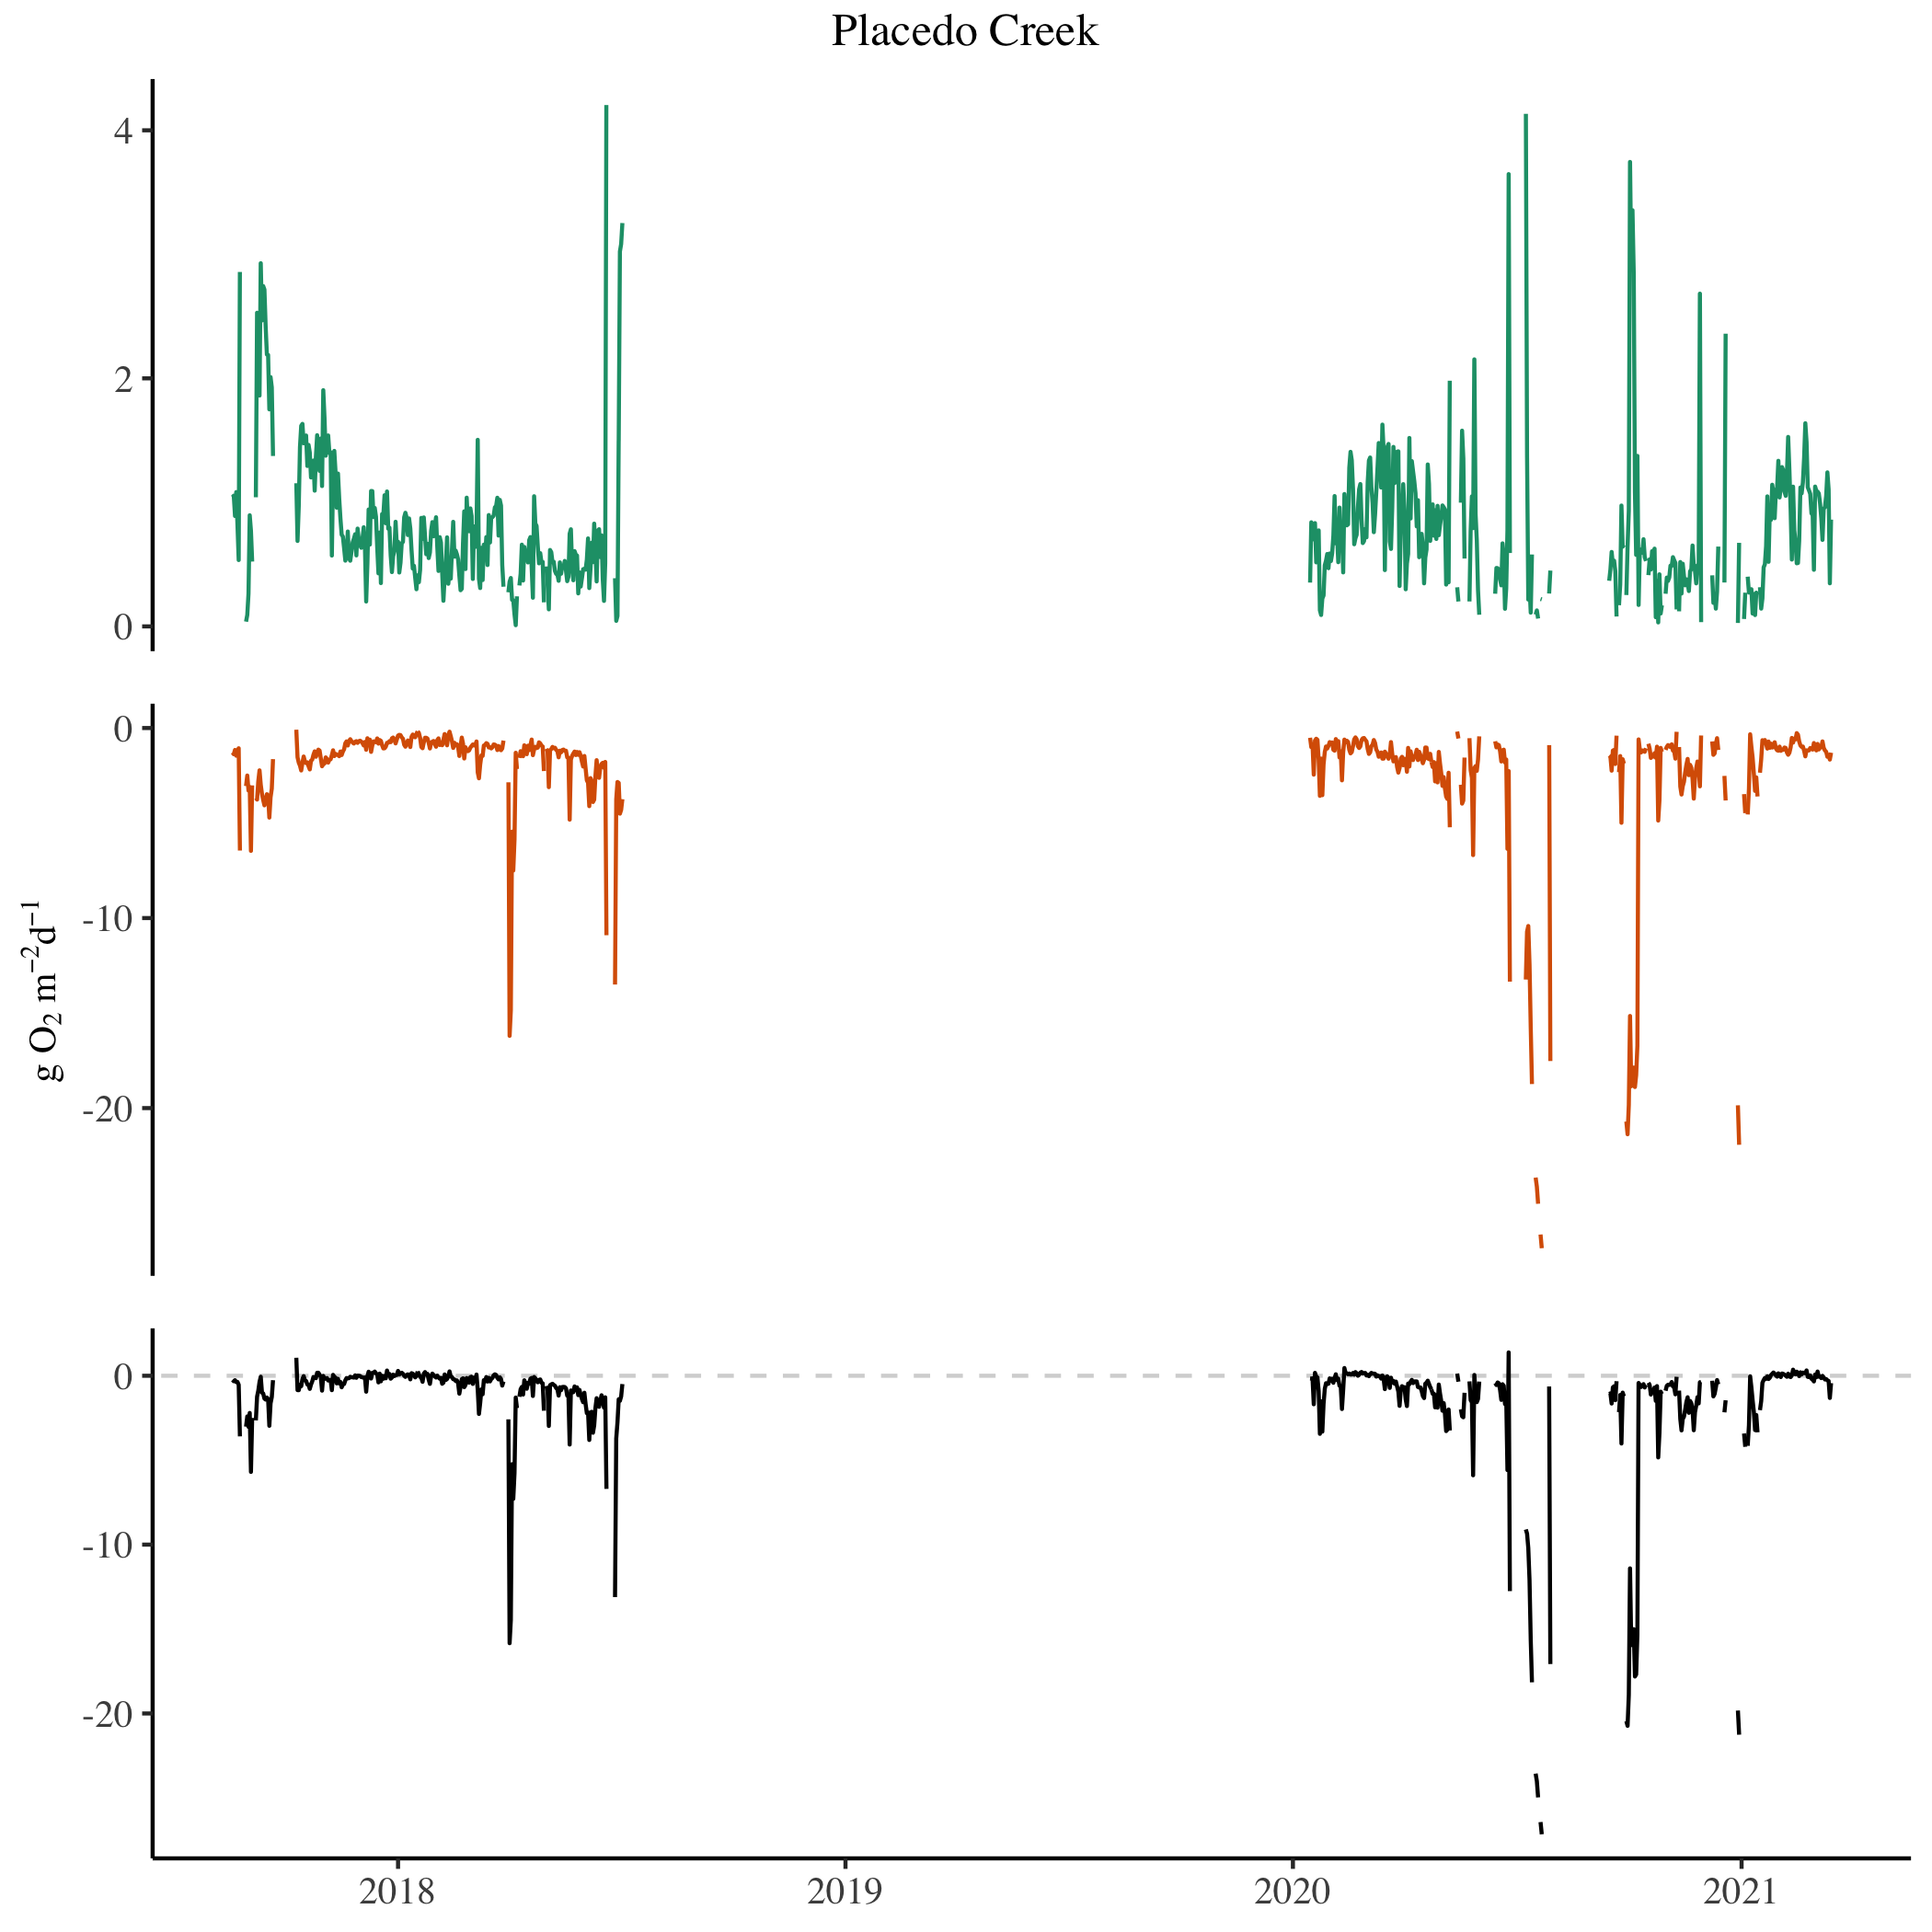
\includegraphics[scale=0.2]{Figs/PLC.png}
\caption{Placedo Creek}
\label{Fig:PLC}
\end{center}
\end{figure}

\begin{figure}[htb]
\begin{center}
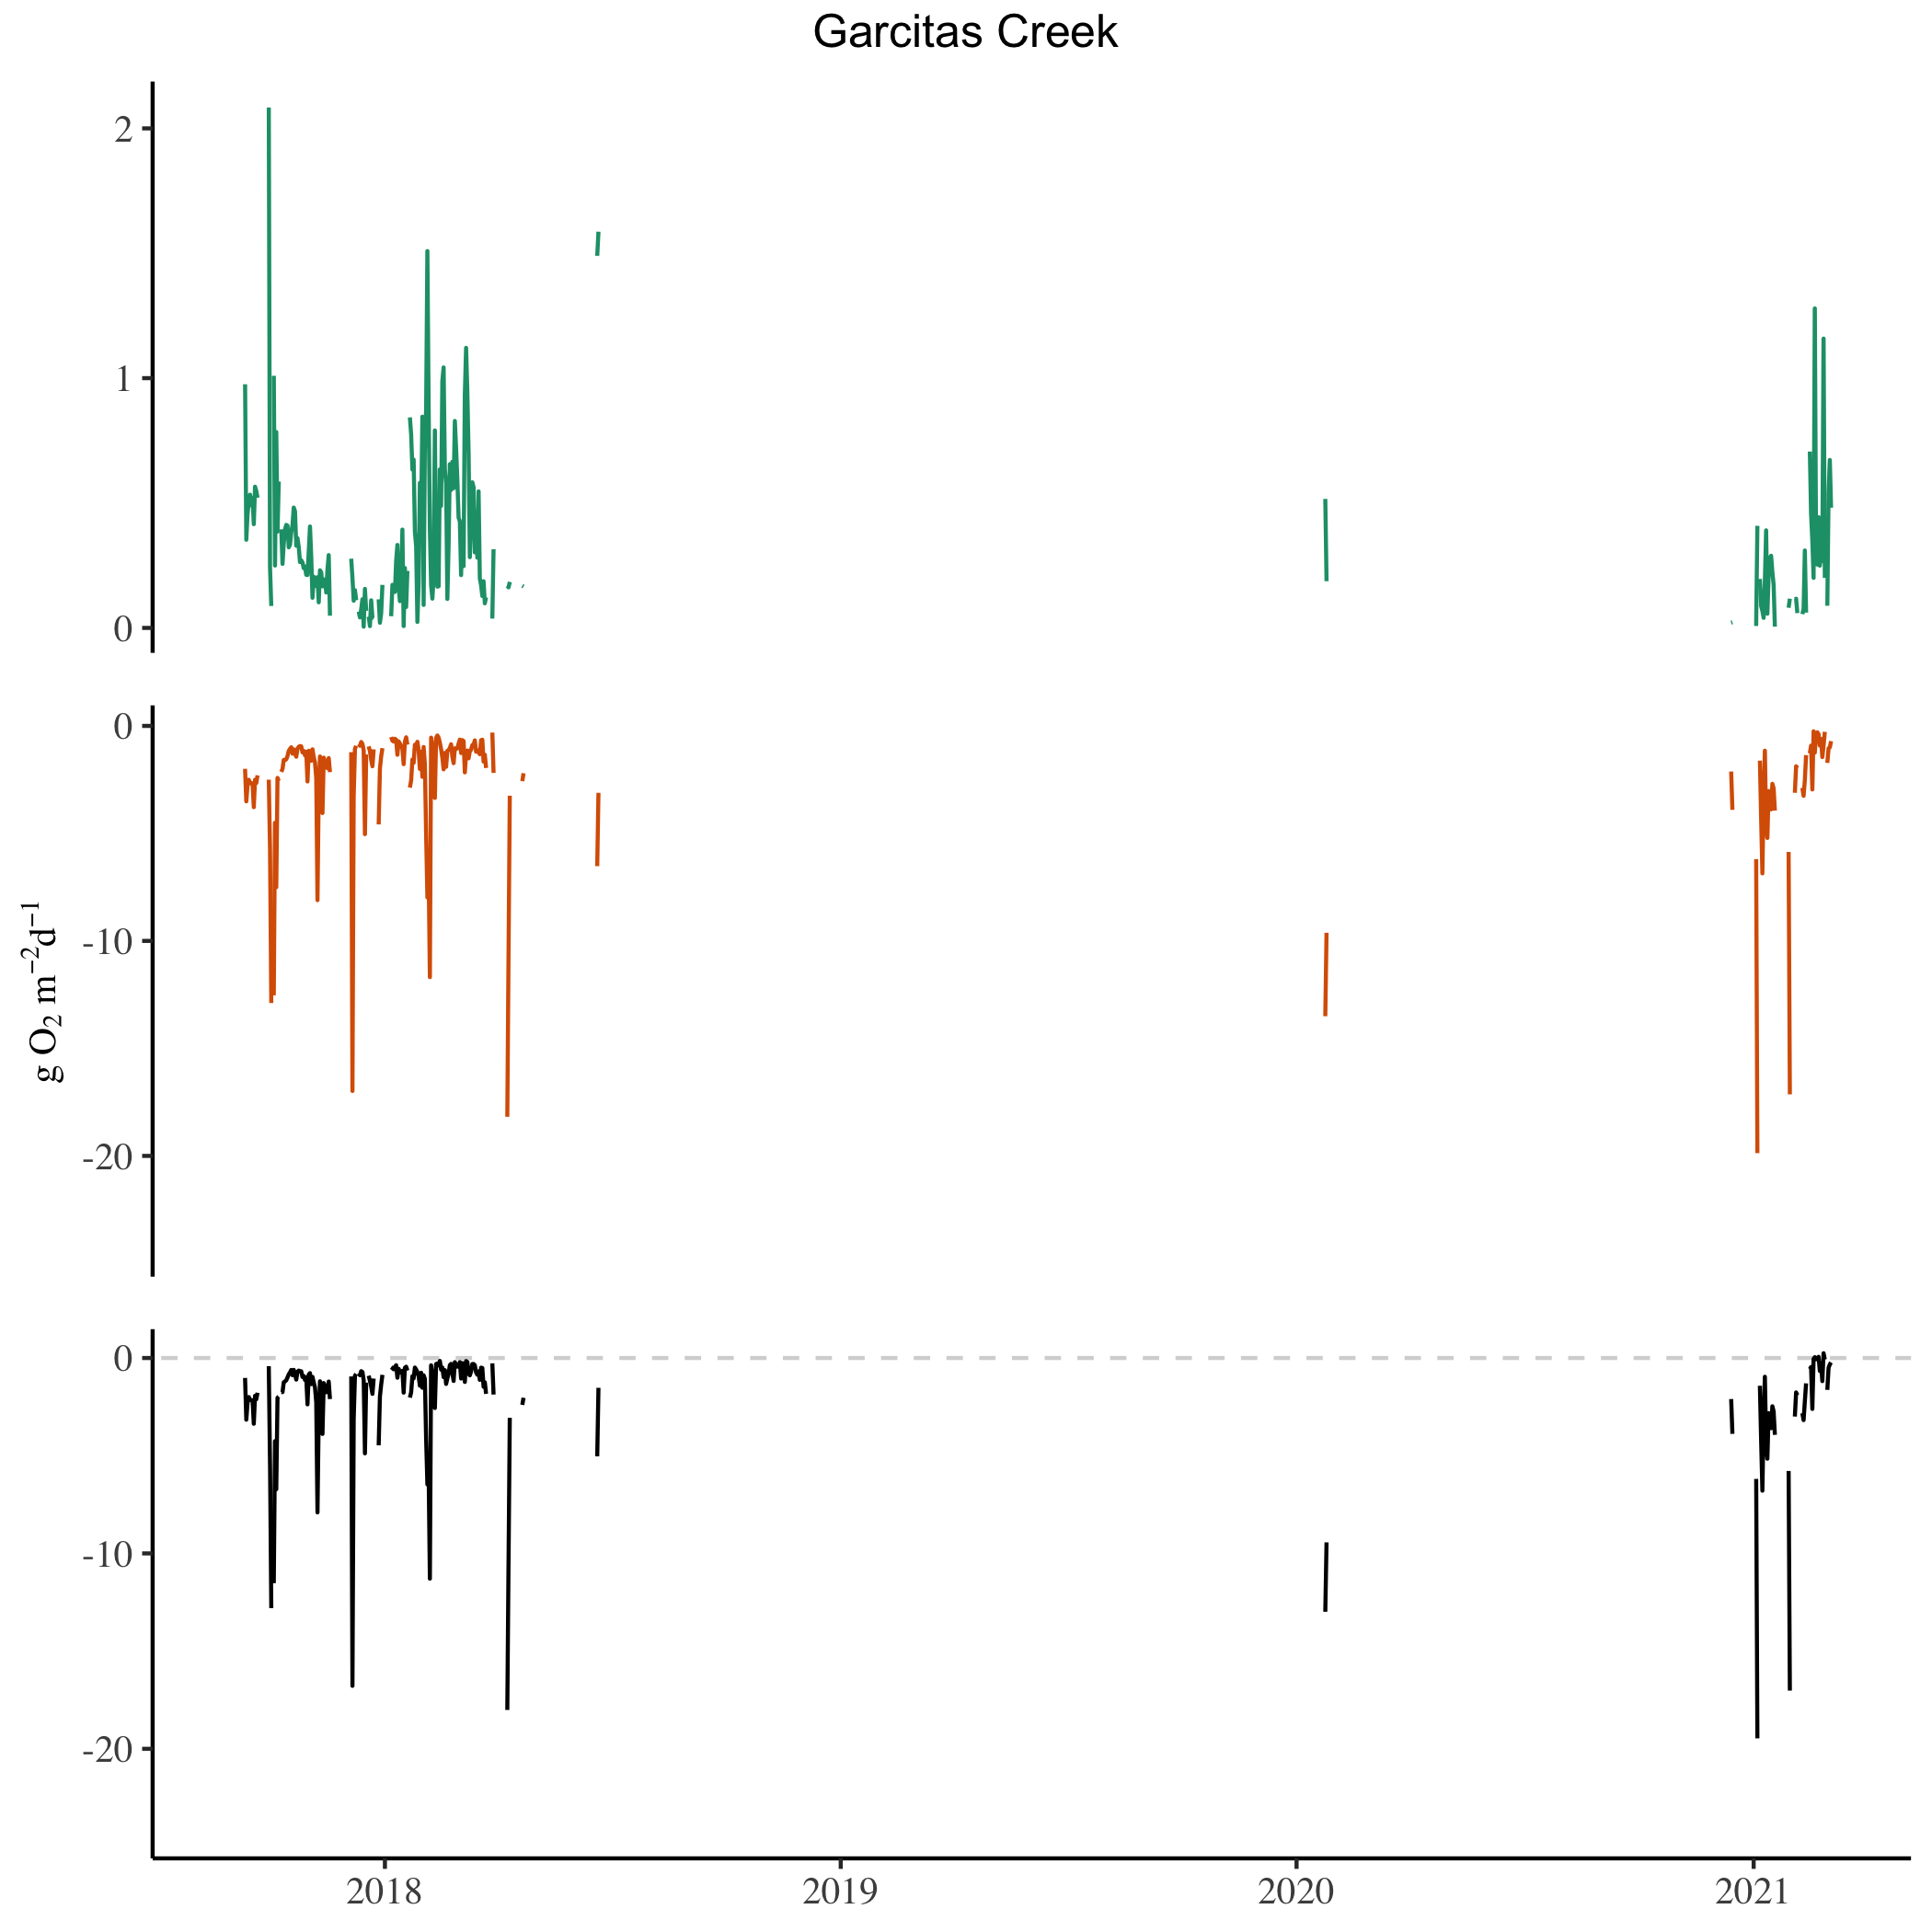
\includegraphics[scale=0.2]{Figs/GC.png}
\caption{Garcitas Creek}
\label{Fig:GC}
\end{center}
\end{figure}

\begin{figure}[htb]
\begin{center}
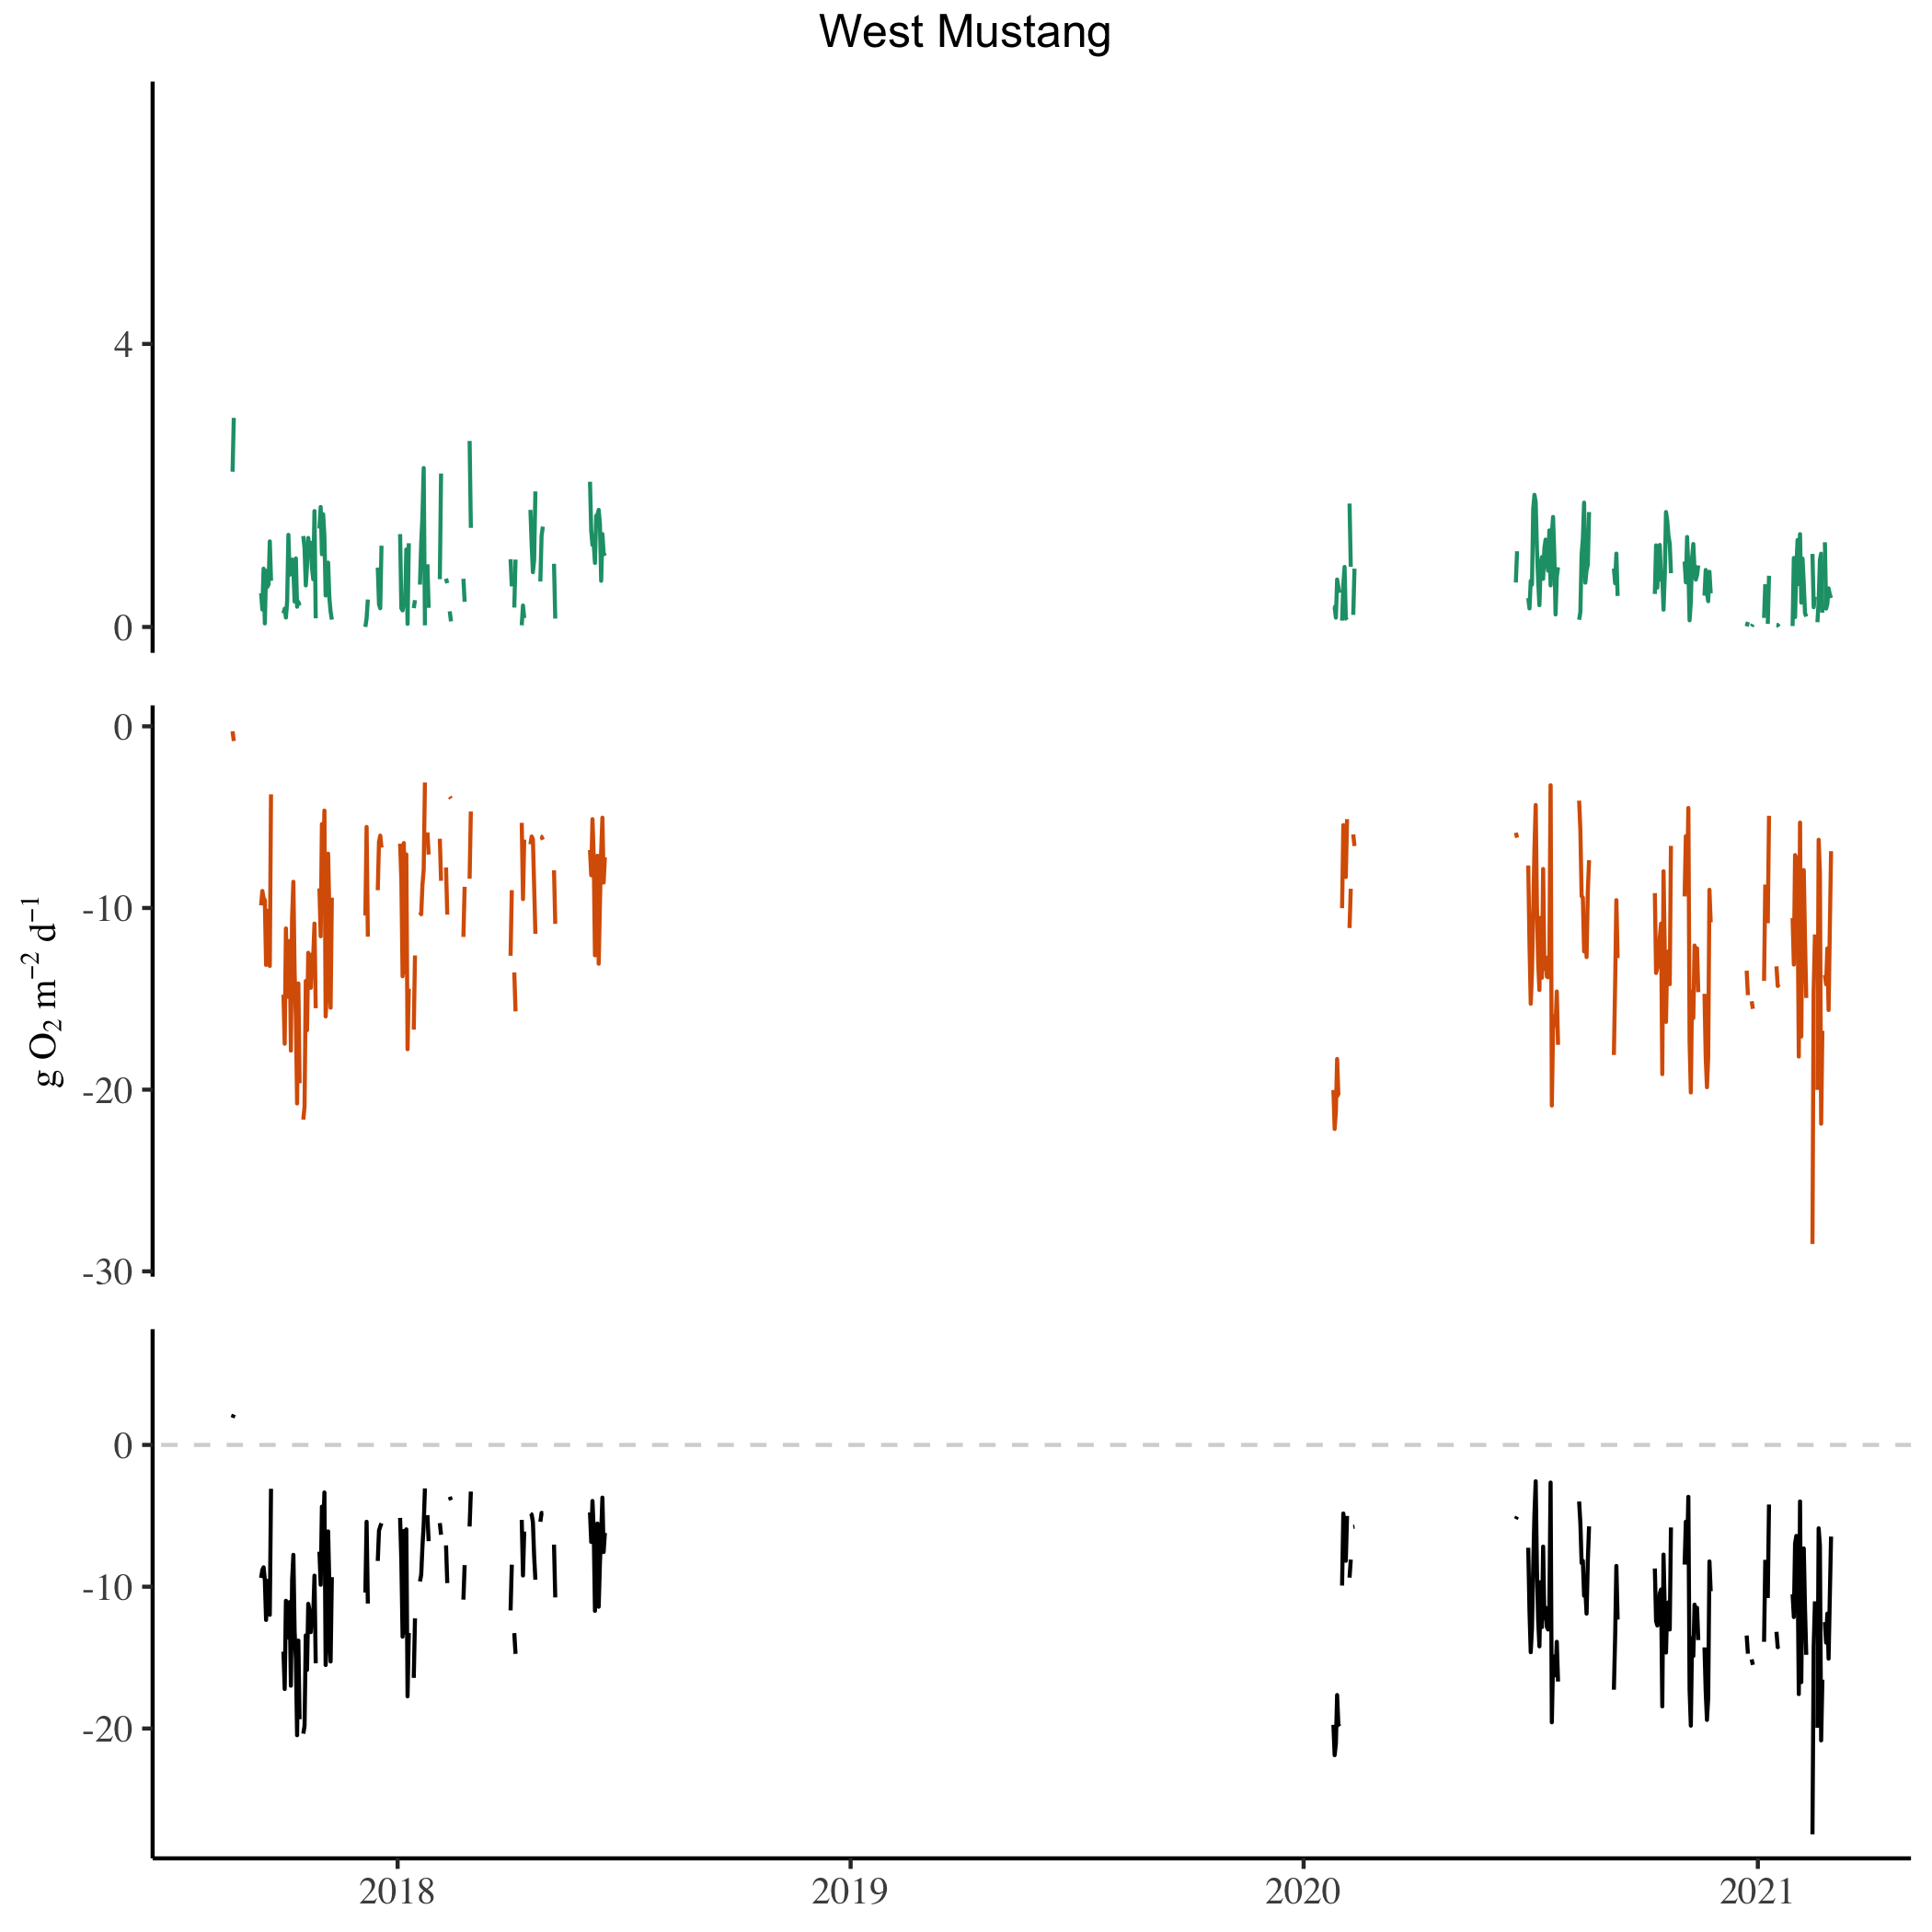
\includegraphics[scale=0.2]{Figs/WMC.png}
\caption{West Mustang Creek}
\label{Fig:WMC}
\end{center}
\end{figure}

\begin{figure}[htb]
\begin{center}
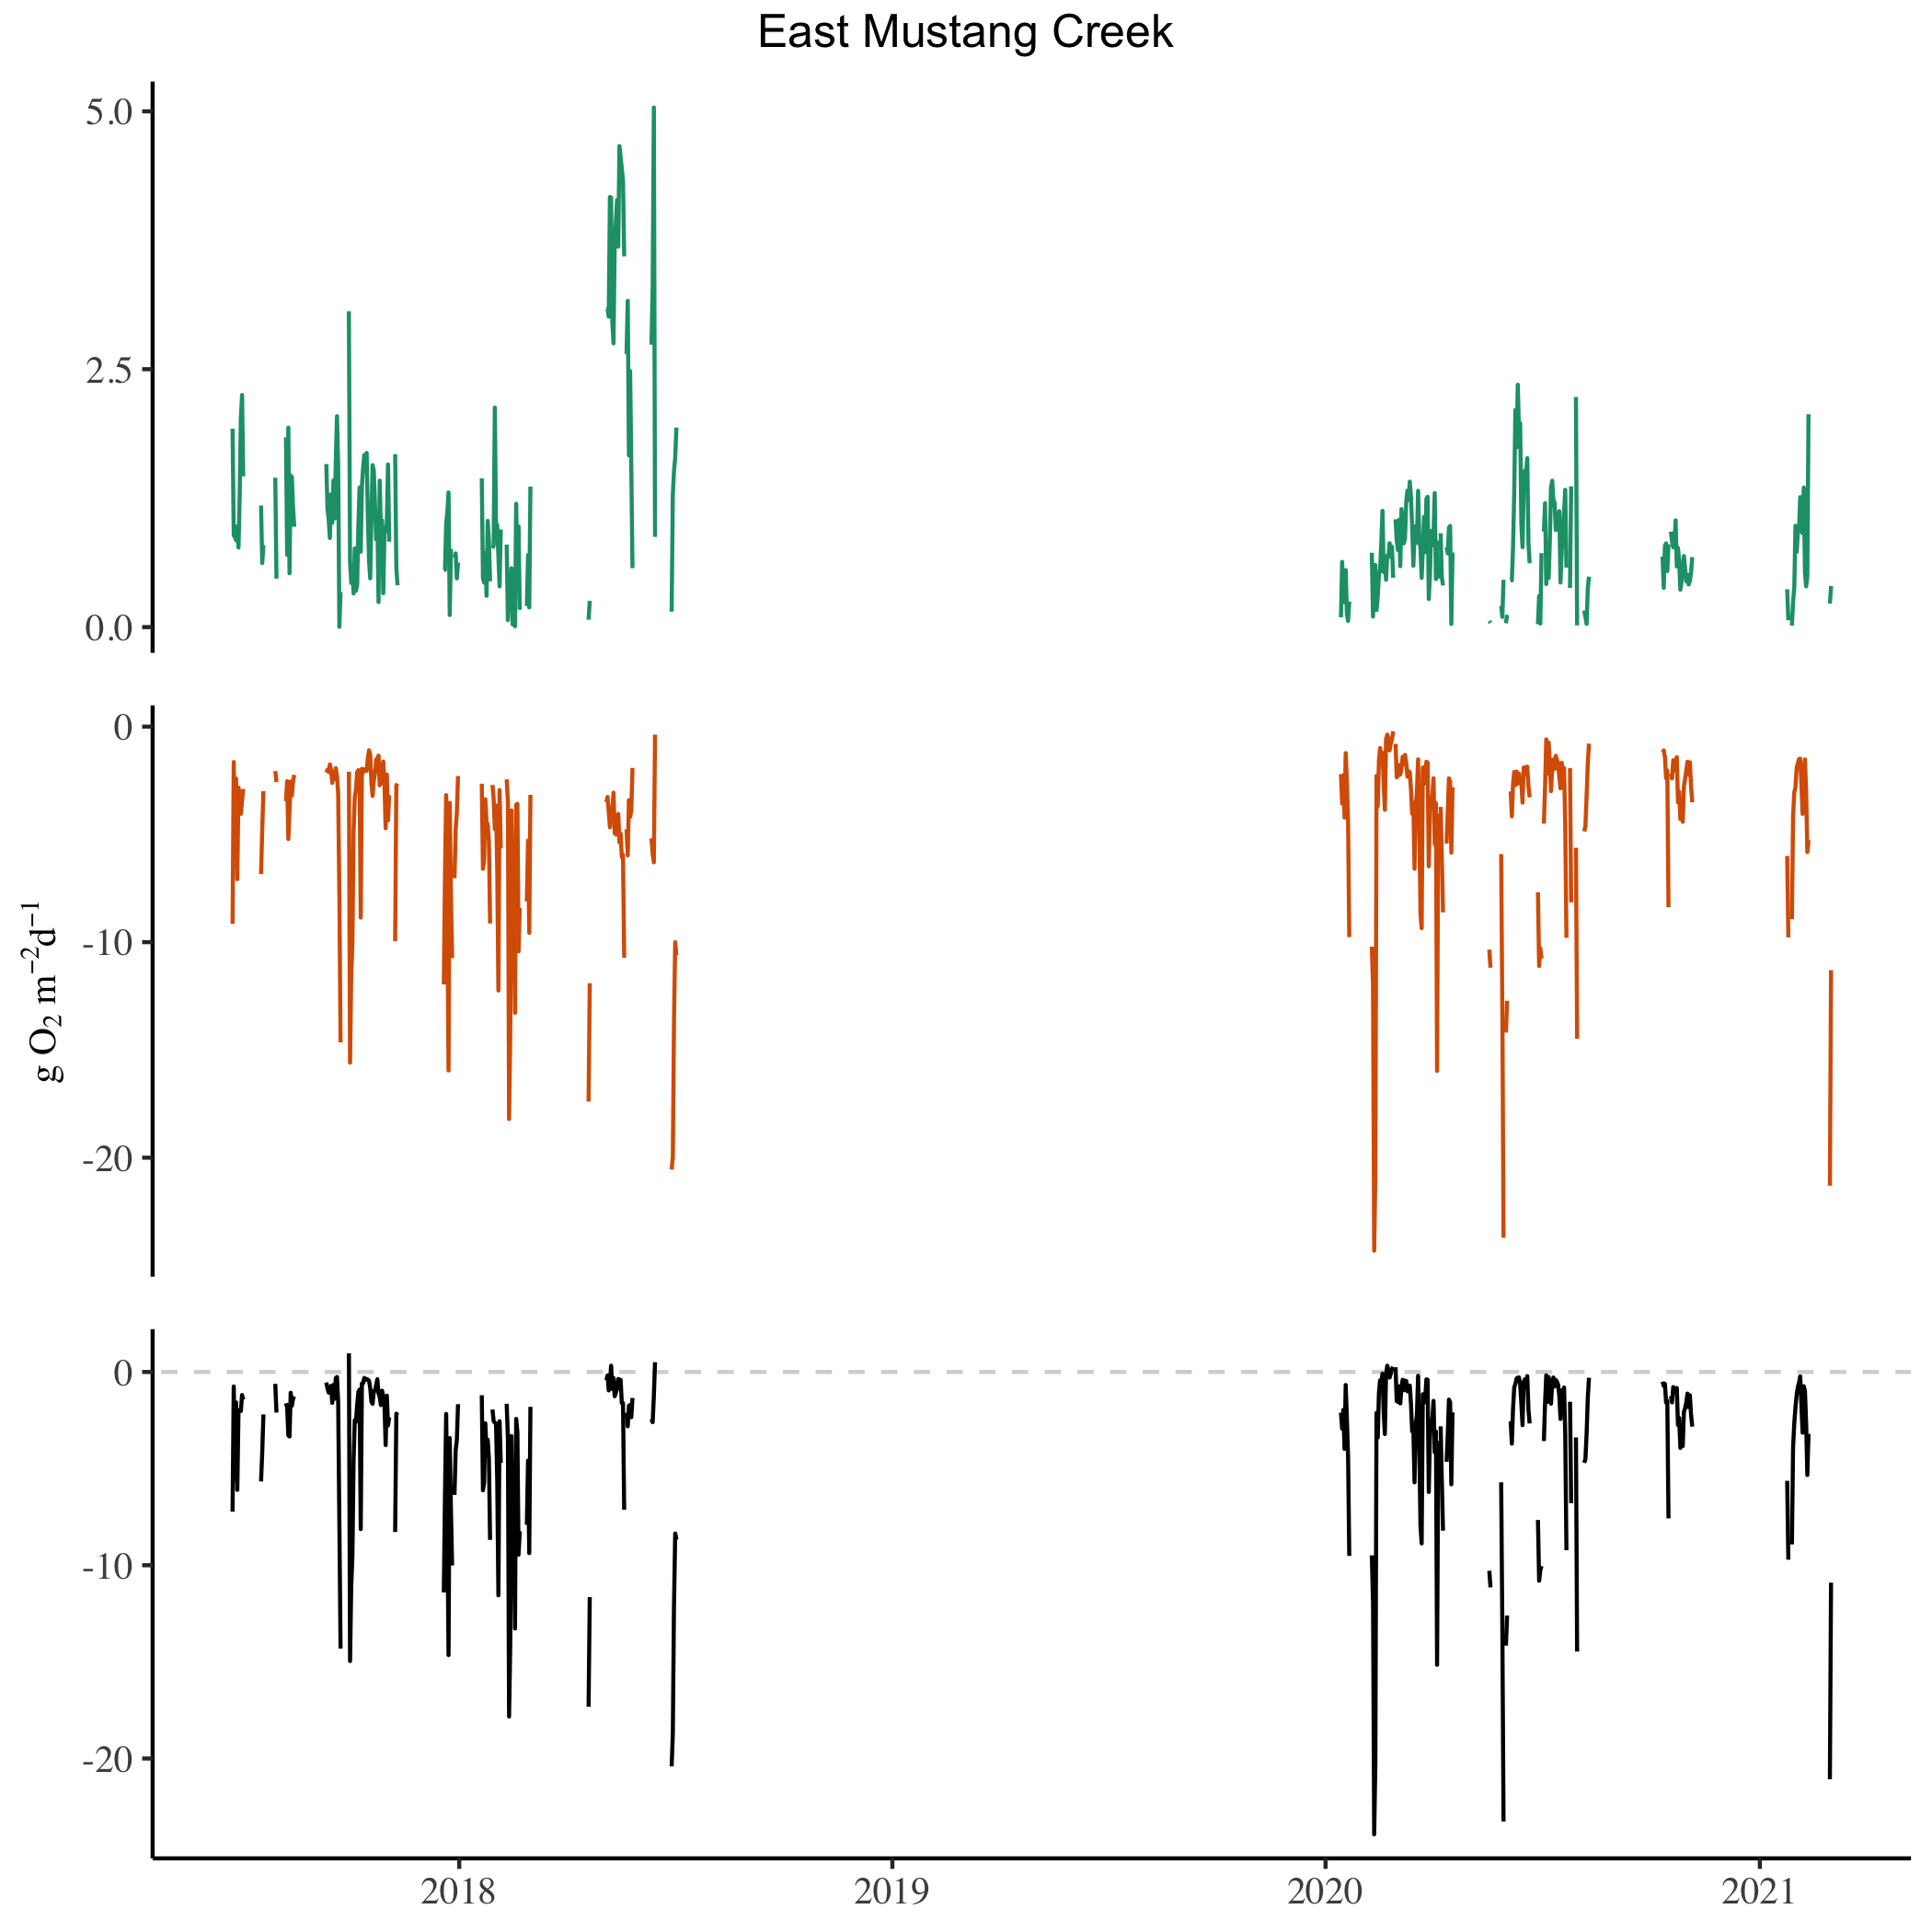
\includegraphics[scale=0.2]{Figs/EMC.png}
\caption{East Mustang Creek}
\label{Fig:EMC}
\end{center}
\end{figure}

\endinput
%-----------------------------------------------------------------------------
% End of appendix1.tex
%-----------------------------------------------------------------------------
